\documentclass[11pt]{article}

\usepackage[margin=1in]{geometry}
\usepackage{amsmath, amssymb}
\usepackage{booktabs}
\usepackage{graphicx}
\usepackage{natbib}
\usepackage{setspace}
\usepackage{hyperref}
\usepackage{caption}

\hypersetup{colorlinks=true, citecolor=blue, linkcolor=blue, urlcolor=blue}
\setlength{\parskip}{0.4em}
\onehalfspacing

% NEW 2026-10-05 (v3): reframed as "The Momentum Mirage" for the MIT Sloan Sports
% Analytics Conference (SSAC 2027). No SSAC formatting guidance is stored in this repo;
% the paper is kept at conference length (11pt, 1in margins, 1.5 spacing).
% Every number in the text comes from data/key_nums_v2.rds (v2 pipeline) or
% data/key_nums_v3.{rds,json} (code/05_mirage_analyses.R). Prose went through the
% accent-write pipeline (stop-slop -> Emulate /humanize -> fact diff); paragraphs where
% Emulate changed meaning or facts keep the pre-Emulate text.
% v2 -> v3 changes:
%   - title, abstract, intro, discussion, conclusion rewritten around four results
%     (bounded null, field-position decomposition, game-FE lesson, cost of chasing momentum)
%   - NEW analyses: Gelbach decomposition, TOST, yards/EP bounds, swing moments,
%     kickoff cost, no-momentum simulation for game FE
%   - FIX: H1 description. v2 text said H1 includes punts after <=3 plays; the v2 code
%     counted all pbp rows, so only 1 punt qualified. H1 is described as what it is and a
%     snap-count version is reported.
%   - Theory section and the full R1-R9 robustness narrative condensed (see paper_v2.tex).

\title{The Momentum Mirage:\\
       \large Field Position, Game Fixed Effects, and the Price of Chasing Swings in the NFL}

\author{Jonathan Walberg\\University of Virginia}
\date{\today}

\begin{document}
\maketitle

\begin{abstract}
\noindent Broadcasters regularly claim that good defensive stops spark the offense to score, and conversely that teams tend to not score following giving up a score. To test this, I fit a series of models for the probability that a team scores on a given drive, using 86,249 drives from 4,078 games from 2010 to 2024 from nflfastR. I find that teams score on 52.3\% of drives following a defensive stop, and 35.6\% of drives otherwise: a 16.7 point difference. Using Gelbach decomposition, I find that 17.0 of these points come from starting field position (defined as the location of the first scrimmage snap of the drive), leaving a residual difference of $-$0.1 points. Including both in the same model, I find a coefficient of $-$0.5 [$-$1.4, 0.4] for defensive stops, and $-$0.6 [$-$1.2, $-$0.0] for being scored on, with equivalence tests allowing me to reject differences of $\pm$2 points (the tightest bound for a stop, 1.42 points, is about 1.7 yards of field position or 0.11 expected points). I also find evidence of carryover from scoring ($+$2.3 points), although simulating a dataset with no momentum indicates about half of this coefficient comes from game-level shocks not absorbed by the model. Finally, I find no evidence that plays that swing momentum (touchdowns of 40+ yards) have a different effect on the following drive than other plays. This paper also contains a lesson about the importance of fixed effects: with only about 21 drives per game, including game fixed effects reduces the coefficient on previous scoring by 5-6 points even when there is no momentum, which caused me to find momentum in earlier versions of this paper. At the end, I show that attempting to exploit momentum through short kickoffs and onside kicks is costly, giving up 0.55 and 0.83 expected points, respectively, relative to a standard kickoff.

\medskip
\noindent\textbf{Keywords:} momentum; hot hand; field position; equivalence tests;
fixed effects; kickoff strategy; nflfastR
\end{abstract}

\section{Introduction}\label{sec:intro}

Momentum is the most quoted and least defined idea in football broadcasting. Within one game you will hear three different claims under the same word. A defense forces a stop and ``gives the offense a spark.'' An offense scores and ``keeps it rolling.'' A team gets scored on and ``can't recover.'' The three claims make different predictions, and the raw numbers seem to back the first one hard: NFL teams score on 52.3\% of drives that follow a defensive stop and on 35.6\% of other drives.

I argue in this paper that this perceived gap is largely a mirage. There is, of course, a mechanical reason stops and takeaways (in particular) lead to points: they put the offense on good field position. Once I account for field position (defined as the location of the first offensive scrimmage), however, the effect shrinks to a relatively tight null: I am able to rule out effects of defensive stops or of being scored on in the previous drive of more than 1.42 percentage points in either direction, a less than two-yard difference in field position.

The paper makes four contributions. First, a Gelbach decomposition shows exactly where the 16.7-point gap goes: 17.0 points to field position, small pieces to the clock and the score, and $-$0.1 points to anything you could call momentum. Second, equivalence tests turn ``not significant'' into a statement with a size attached, priced in yards and expected points with the model's own slopes. Third, the plays fans remember as momentum swings (takeaways, fourth-down stops, long touchdowns, defensive and return touchdowns) do not move the next drive beyond what an ordinary score or stop does. Fourth, a methods lesson: with about 21 drives per game, game fixed effects manufacture large negative lagged effects. An earlier version of this analysis reported a 32.7-point ``opponent suppression'' effect that came from that bias combined with a field-position coding error. Finally, I price the decision that follows from believing in momentum. Short kickoffs and onside kicks after scores cost the kicking team between half a point and nearly a full point of expected value.

\section{Related Literature}\label{sec:lit}

The hot-hand debate starts with \citet{gilovich1985hot}, who found that basketball shooting streaks look like independent draws. \citet{miller2018surprised} showed that the original test carried a selection bias and that, once corrected, modest streak effects appear. \citet{bareli2006twelve} review the sport-psychology literature that treats momentum as a real psychological state. In team sports the unit of analysis matters. \citet{stern1994probabilities} models score progression as Brownian motion. \citet{berger2011hot} find that trailing slightly at halftime raises the chance of winning in the NBA and NCAA basketball, which they read as an effort response. \citet{csapo2014hand} show that NBA defenses adjust to perceived hot hands, and \citet{gauriot2019does} find momentum between players in professional tennis.

For the NFL, \citet{fry2012searching} test game-to-game momentum and find none beyond team strength. \citet{arkes2011finally} report modest game-to-game carryover in the NBA, \citet{steeger2021winning} find NHL win sequences consistent with chance, and \citet{lopez2018often} show that NFL outcomes carry more randomness than outcomes in the other three major North American leagues. None of these studies works at the drive level, where coaches make the in-game call. The tools for a drive-level test come from \citet{yurko2018nflwar} and the nflfastR package \citep{nflfastr2024}. Drive-level work includes Markov models of drive progression \citep{goldner2012markov}, third-down analysis \citep{cafarelli2012third}, win-probability models \citep{lock2014random}, fourth-down decisions \citep{yam2019what}, and expected-points estimation \citep{brill2024expected}.

\section{Data and Design}\label{sec:data}

The data are nflfastR play-by-play for regular-season and postseason games from 2010 through 2024 \citep{nflfastr2024}. I aggregate plays to drives with the \texttt{fixed\_drive} identifier and drop end-of-half and end-of-game drives, leaving 86,249 drives in 4,078 games. A drive succeeds if it ends in a touchdown or field goal. I define three lagged indicators from the point of view of the team with the ball. H1 (defensive stop) equals one if the opponent's immediately preceding drive ended in an interception, a lost fumble, a turnover on downs, or a safety. H2 (offensive carryover) equals one if the team's own previous offensive drive scored. H3 (opponent suppression) equals one if the opponent's previous drive scored. Requiring all three leaves 74,125 drives, and 74,120 have the clock variable.

Two measurement choices drive the results. The first is field position. nflfastR files the kickoff as the first row of the receiving team's drive, so a drive's first row after an opponent score records the kicking spot, the 35, rather than where the offense lines up. Version 1 of this analysis used that first row and coded 91.9\% of post-score drives as starting on the opponent's 35. I take field position from the offense's first scrimmage snap. Drives that follow an opponent score start 74.9 yards from the end zone on average, against 69.3 yards for other drives.

The second choice was on the definition of a stop. Earlier versions of this project had H1 stops as including punts after three or fewer plays. The code I used to write this tabulated every play-by-play row in the game (so including kickoffs, timeouts, quarter breaks, etc.) and so only one punt made it into the indicator. The H1 indicator is, effectively, a takeaway indicator, with 11,824 drives that began after a turnover, turnover on downs, or safety. I’ll leave that as the headline indicator so that I can compare to earlier versions of the project, but will also include the snap count version, which includes 18,652 three-and-out punts, for a total of 30,475 stop drives.

The headline model is a linear probability model that regresses drive success on the three indicators of interest, the team’s starting field position, the score differential, the quarter, the number of seconds remaining in the half, and an indicator for whether the possessing team is playing at home. I also include fixed effects for the possessing team, fixed effects for the opponent, and fixed effects for the season. Standard errors are two-way clustered by game and by the team in possession \citep{cameron2011robust}. I exclude game fixed effects from the headline model for reasons explained in Section~\ref{sec:fe}.

\begin{table}[htbp]
\centering
\caption{Unconditional drive-level scoring probabilities by prior context.}
\label{tab:descrip}
\begin{tabular}{lcc}
\toprule
Condition & P(score) & N drives \\
\midrule
After own defensive stop & 0.523 & 11,824 \\
After opponent score or longer punt & 0.356 & 66,378 \\
\midrule
After own offensive score (prior own drive) & 0.403 & 28,625 \\
After own offensive non-score & 0.370 & 49,554 \\
\midrule
After opponent score (prior opp drive) & 0.352 & 31,193 \\
After opponent non-score & 0.400 & 50,910 \\
\bottomrule
\end{tabular}
\\[0.5em]
\begin{minipage}{0.95\textwidth}
\footnotesize
\textit{Notes.} Each panel uses the largest sample for which the relevant prior-drive indicator is defined; sample size therefore differs across panels (the unified estimation sample requiring all three indicators is N = 
74{,}125
 drives). Sample: NFL regular season + postseason 2010--2024 from nflfastR. 
\end{minipage}
\end{table}


\section{The Gap Is Field Position: A Bounded Null}\label{sec:results}

Figure~\ref{fig:fp} shows the gap disappearing. Within each field-position decile, drives after a stop and drives after any other opponent outcome score at nearly the same rate. Table~\ref{tab:decomp} puts numbers on the picture with a \citet{gelbach2016covariates} decomposition, which splits the change in the stop coefficient between the raw comparison and the full model into the part each block of controls explains. Field position explains 17.0 points of the 16.7-point gap, or 102\%. The clock takes away 0.3 points and the score margin 0.1, the possessing-team fixed effects add 0.2, and the stop coefficient in the full model is $-$0.1 points (s.e. 0.5). On the joint-model sample the raw gap is 16.3 points, field position explains 16.8 of them, and the residual is the $-$0.5 reported below.

\begin{figure}[htbp]
\centering
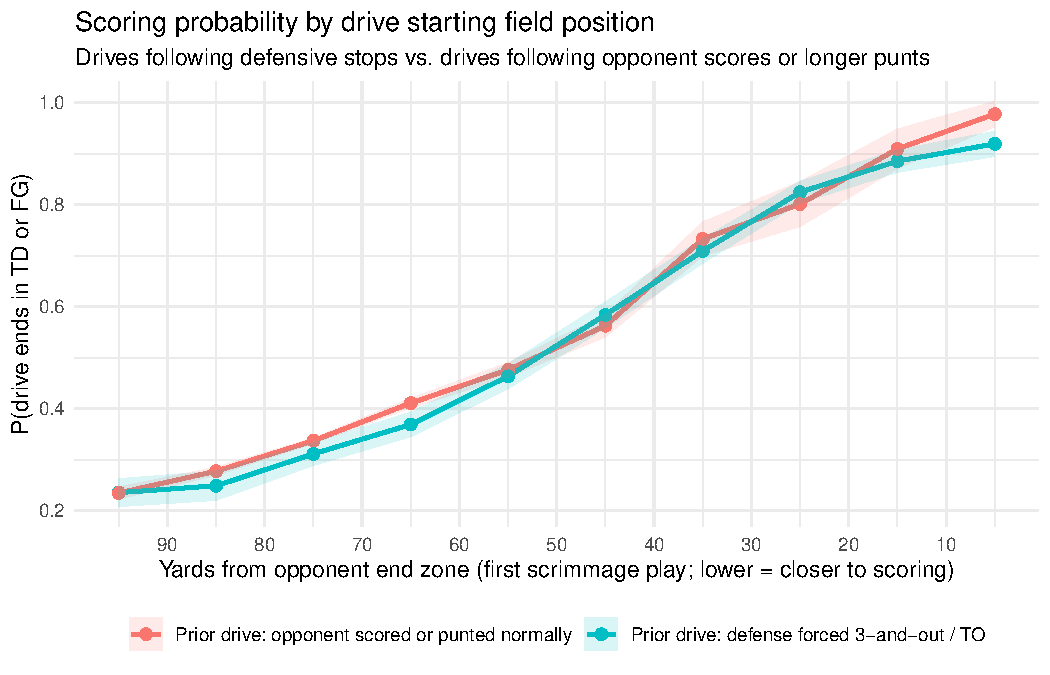
\includegraphics[width=0.8\textwidth]{figures/fig1_field_position_v2.pdf}
\caption{Scoring probability by starting field position decile (yards from the opponent
end zone at the first scrimmage snap), for drives after a defensive stop (solid) and after
any other opponent outcome (dashed). Drives with the H1 indicator defined (78{,}202),
NFL 2010--2024, \texttt{nflfastR}. Bands are 95\% binomial intervals.}
\label{fig:fp}
\end{figure}

{\small\setlength{\tabcolsep}{4pt}\begin{table}[htbp]
\centering
\caption{\label{tab:decomp} Where the defensive-stop gap goes: Gelbach (2016) decomposition. Percentage points. The raw gap is the difference in scoring rates after a defensive stop versus any other opponent outcome (N = 78,197 drives with the H1 indicator and time remaining). Each row is the part of the gap explained by that block of the headline specification (field position, score differential, quarter and half-seconds remaining, home, and possessing-team, opponent, and season fixed effects). Bootstrap standard errors (200 game-cluster resamples) in parentheses. Shares are of the raw gap.}
\begin{tabular}{lrrr}
\toprule
Component & Estimate (pp) & (s.e.) & Share (\%) \\
\midrule
Raw gap (stop minus no stop) & 16.7 & (0.5) & 100 \\
\midrule
Field position & 17.0 & (0.3) & 102 \\
Score state & -0.1 & (0.1) & -1 \\
Time remaining & -0.3 & (0.0) & -2 \\
Home & 0.0 & (0.0) & 0 \\
Possessing-team FE & 0.2 & (0.0) & 1 \\
Opponent FE & 0.0 & (0.0) & 0 \\
Season FE & 0.0 & (0.0) & 0 \\
\midrule
Residual (H1 coefficient, full spec) & -0.1 & (0.5) & -1 \\
\bottomrule
\end{tabular}
\end{table}
}

\begin{figure}[htbp]
\centering
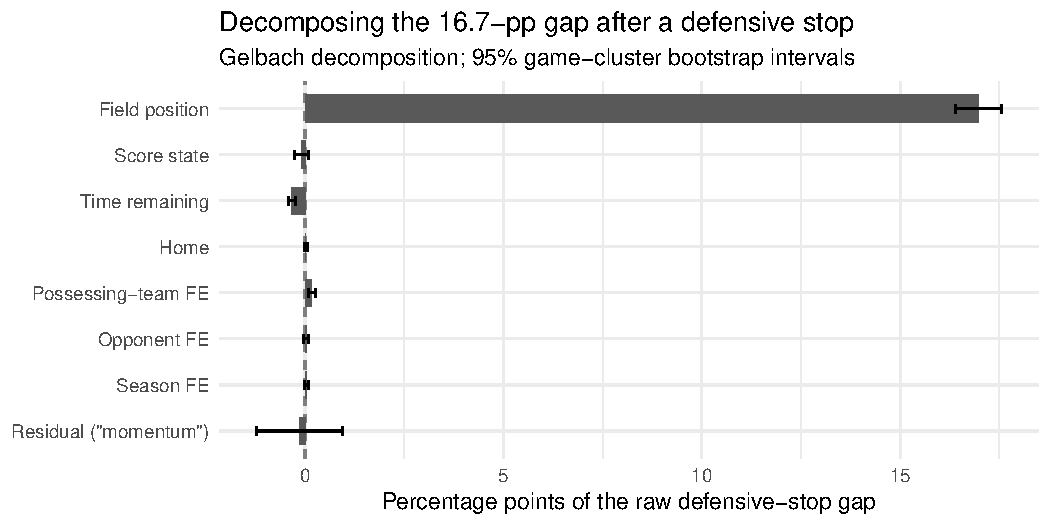
\includegraphics[width=0.8\textwidth]{figures/fig3_decomp_v3.pdf}
\caption{Gelbach decomposition of the defensive-stop gap (Table \ref{tab:decomp}).
Bars are percentage points of the raw gap; whiskers are 95\% game-cluster bootstrap intervals.}
\label{fig:decomp}
\end{figure}

Table~\ref{tab:allchan} reports the joint model. The H1 coefficient is $-$0.5 points (s.e. 0.6, $p=0.39$), H2 is $+$2.3 (s.e. 0.4), and H3 is $-$0.6 (s.e. 0.3, $p=0.09$). A null result needs a size before it means anything, so Table~\ref{tab:tost} runs two one-sided equivalence tests \citep{lakens2017equivalence} against bounds of $\pm$2 and $\pm$1 points. For H1 the 90\% interval runs from $-$1.4 to 0.4. The test rejects effects outside $\pm$2 points ($p=0.004$) but not outside $\pm$1 ($p=0.18$), and the tightest bound it supports is 1.42 points. For H3 the interval runs from $-$1.2 to $-$0.0, the test rejects effects outside $\pm$2 points ($p<0.001$), and the tightest bound is 1.17 points.


\begin{table}[htbp]
   \caption{\label{tab:allchan} Three Momentum Channels: Joint Estimation and Robustness. Field position is the yardline of the offense's first scrimmage play. \textit{Notes.} Column 1 is the preferred specification: linear probability model for whether the drive ends in a score, with all three momentum indicators jointly. Column 2 drops drives in garbage time (absolute score differential $\geq 21$ in the fourth quarter). Column 3 replaces the binary outcome with the sum of expected-points-added (EPA) on the drive. All columns include game-state controls (field position, score differential, quarter, half-seconds remaining, home indicator) and possessing-team, opponent, and season fixed effects. Standard errors in parentheses, two-way clustered by game and possessing team \citep{cameron2011robust}. $^{*}p<0.10$, $^{**}p<0.05$, $^{***}p<0.01$.}
   \centering
   \begin{tabular}{lccc}
      \tabularnewline \midrule \midrule
      Dependent Variables: & \multicolumn{2}{c}{Drive ends in score (0/1)} & Drive EPA\\
      Model:                                  & (1)                           & (2)                           & (3)\\  
      \midrule
      \emph{Variables}\\
      Prior own defensive stop                & -0.0049                       & -0.0025                       & -0.2852$^{***}$\\   
                                              & (0.0056)                      & (0.0058)                      & (0.0432)\\   
      Prior own offensive score               & 0.0229$^{***}$                & 0.0207$^{***}$                & 0.1623$^{***}$\\   
                                              & (0.0043)                      & (0.0041)                      & (0.0331)\\   
      Prior opponent offensive score          & -0.0060$^{*}$                 & -0.0049                       & 0.0006\\   
                                              & (0.0035)                      & (0.0035)                      & (0.0347)\\   
      Field position (yards to opp. end zone) & -0.0082$^{***}$               & -0.0081$^{***}$               & -0.0075$^{***}$\\   
                                              & (0.0001)                      & (0.0001)                      & (0.0009)\\   
      Score differential                      & -0.0005$^{***}$               & -0.0001                       & -0.0022\\   
                                              & (0.0002)                      & (0.0002)                      & (0.0014)\\   
      Quarter                                 & -0.0113$^{***}$               & -0.0080$^{***}$               & -0.0914$^{***}$\\   
                                              & (0.0015)                      & (0.0016)                      & (0.0106)\\   
      Half seconds remaining                  & $2.08\times 10^{-5}$$^{***}$  & $1.66\times 10^{-5}$$^{***}$  & $-9.33\times 10^{-6}$\\    
                                              & ($3.54\times 10^{-6}$)        & ($3.46\times 10^{-6}$)        & ($2.8\times 10^{-5}$)\\    
      Home offense                            & 0.0228$^{***}$                & 0.0219$^{***}$                & 0.0243\\   
                                              & (0.0037)                      & (0.0039)                      & (0.0269)\\   
      \midrule
      \emph{Fixed-effects}\\
      Possessing team                         & Yes                           & Yes                           & Yes\\  
      Opponent                                & Yes                           & Yes                           & Yes\\  
      Season                                  & Yes                           & Yes                           & Yes\\  
      \midrule
      \emph{Fit statistics}\\
      Observations                            & 74,120                        & 71,368                        & 74,120\\  
      R$^2$                                   & 0.09089                       & 0.09078                       & 0.01039\\  
      Within R$^2$                            & 0.08262                       & 0.08235                       & 0.00240\\  
      \midrule \midrule
      \multicolumn{4}{l}{\emph{Clustered (Game \& Possessing team) standard-errors in parentheses}}\\
      \multicolumn{4}{l}{\emph{Signif. Codes: ***: 0.01, **: 0.05, *: 0.1}}\\
   \end{tabular}
\end{table}




{\footnotesize\setlength{\tabcolsep}{3pt}\begin{table}[htbp]
\centering
\caption{\label{tab:tost} Equivalence tests (two one-sided tests, $\alpha=0.05$). Estimates from the headline specification (column 1 of Table \ref{tab:allchan}). $p_{\pm b}$ is the TOST $p$-value against the equivalence bound $\pm b$ percentage points; $p<0.05$ means the effect is shown to lie inside the bound. The smallest bound is the tightest $\pm b$ the 90\% interval rules out. Yards convert that bound with the model's own field-position slope (0.82 pp per yard); expected points (EP) convert the yards with the slope of \texttt{nflfastR} EP at the first scrimmage play (0.061 EP per yard).}
\begin{tabular}{lccccccc}
\toprule
 & Est. (s.e.), pp & 90\% CI & $p_{\pm 2}$ & $p_{\pm 1}$ & Smallest bound (pp) & Yards & EP \\
\midrule
H1 & -0.5 (0.6) & [-1.4, 0.4] & 0.004 & 0.183 & 1.42 & 1.74 & 0.11 \\
H2 & 2.3 (0.4) & [1.6, 3.0] & 0.751 & 0.999 & 2.99 & 3.66 & 0.23 \\
H3 & -0.6 (0.3) & [-1.2, -0.0] & $<$0.001 & 0.124 & 1.17 & 1.43 & 0.09 \\
\midrule
\multicolumn{8}{l}{\emph{Stops counted on scrimmage snaps (three-and-out punts included)}} \\
H1 (snap-count stops) & -1.3 (0.4) & [-2.0, -0.6] & 0.040 & 0.733 & 1.96 & 2.40 & 0.15 \\
H2 (same model) & 2.3 (0.4) & [1.6, 3.0] & 0.740 & 0.999 & 2.97 & 3.64 & 0.22 \\
H3 (same model) & -1.2 (0.4) & [-1.9, -0.6] & 0.023 & 0.727 & 1.86 & 2.28 & 0.14 \\
\bottomrule
\end{tabular}
\end{table}
}

The model's own slopes translate those bounds. Each yard of starting field position moves scoring probability by 0.82 points, and in nflfastR each yard is worth 0.061 expected points at the first snap. The H1 bound equals 1.74 yards and 0.11 expected points. The H3 bound equals 1.43 yards and 0.09 expected points. Put another way, any momentum from a takeaway or from being scored on is smaller than the value of a two-yard difference in where the offense starts.

The only channel that clears zero is H2, which has a 90\% interval between 1.6 and 3.0 points. However, the equivalence test p-value is still large (0.75), meaning that the test does not rule out an effect of 2 points. The upper bound of the interval is 2.99 points, 3.66 yards, or 0.23 expected points. As discussed in Section~\ref{sec:fe} , part of the estimated momentum comes from the fact that scoring teams score on a lot of drives (i.e. they're having a good day), so a simulation with no momentum still gives a headline model estimated momentum of $+$1.2 points for H2.

The snap-count stop definition does not rescue momentum. Adding three-and-out punts shrinks the raw gap to 10.0 points (44.3\% against 34.2\%), and the adjusted stop coefficient turns slightly negative at $-$1.3 points (s.e. 0.4, 90\% CI $-$2.0 to $-$0.6). The equivalence test still rejects effects outside $\pm$2 points ($p=0.04$). H3 in that model is $-$1.2 points (s.e. 0.4), with a tightest bound of 1.86 points. Under either definition, nothing points to a positive spark after a stop.

The bounded null survives the checks from the earlier version, which all use the corrected field position. Flexible field-position and score controls give $-$1.6, $+$2.4, and $-$0.2 points for H1 to H3. Logit average marginal effects are $-$0.3, $+$0.8, and $-$0.0. Dropping garbage time gives $-$0.3, $+$2.1, and $-$0.5. A permutation test places the observed H3 inside its null distribution ($p=0.09$), and H3 stays between $-$1.7 and $-$0.7 points in each of four kickoff-rule eras.

\section{Momentum-Swing Moments}\label{sec:swing}

On the football field, it’s said that football fans don’t remember three and outs, but they do remember spectacular plays. Thus, if momentum exists it should exist after spectacular plays. Table~\ref{tab:swing} looks at the possession of the opponent prior to the team’s possession and then uses the headline controls to identify the probability of scoring on the following drive. The comparison group is opponent drives that resulted in a longer punt, a missed field goal or other non-scoring result.

The swing plays do not swing the next drive. After a takeaway the offense scores 0.7 points more often than after the reference outcome (s.e. 0.7), and 2.0 points more than after a three-and-out (s.e. 0.7). A long touchdown against you, with a scoring play of 40 yards or more, lowers your next drive's scoring rate by 1.3 points, exactly what a short touchdown does: the difference is 0.0 points (s.e. 1.3). A defensive or return touchdown against you is no worse than a short offensive touchdown (difference 0.2, s.e. 1.1). The team that made the big play gains nothing on its own next possession either. After its own long touchdown it scores 0.1 points less than after a shorter touchdown (s.e. 1.2), and after its defense or return unit scores, 0.1 points less (s.e. 1.6).

There is one obvious swing play that jumps out at the top of the list. When the defense makes a stop on 4th down, the offense scores 5.4 points less often (s.e. 0.8) than they do following whatever the reference outcome was. This is likely not due to a weak offense, since a lot of 4th down stops come late in the game when the opposition is going for it because they are behind and this team has a lead to protect. Instead, this is likely due to the effect of game situation which is not controlled for in this linear specification.

{\small\setlength{\tabcolsep}{4pt}\begin{table}[htbp]
\centering
\caption{\label{tab:swing} Scoring after momentum-swing moments. Percentage-point change in the probability that the next drive ends in a score, from linear probability models with the headline controls (field position at the first scrimmage play, score differential, quarter, half-seconds remaining, home) and possessing-team, opponent, and season fixed effects. Panel A: categories of the opponent possession immediately before the drive; reference category is an opponent drive ending in a punt after four or more plays, a missed field goal, or another non-scoring outcome (N = 79,367). Panel B: the team that made the big play, on its next offensive drive, also controlling for whether its previous drive was a touchdown and whether the opponent just scored (N = 78,004). Standard errors two-way clustered by game and possessing team.}
\begin{tabular}{lrrr}
\toprule
Preceding event & Est. (pp) & (s.e.) & N \\
\midrule
\multicolumn{4}{l}{\emph{A. Drive right after the event}} \\
Takeaway (INT or fumble lost) & 0.7 & (0.7) & 8,660 \\
Fourth-down stop & -5.4 & (0.8) & 2,942 \\
Punt after $\leq$3 scrimmage snaps, or safety & -1.3 & (0.4) & 18,872 \\
Opponent field goal & -0.8 & (0.6) & 11,467 \\
Opponent offensive TD, scoring play $<$40 yds & -1.3 & (0.5) & 15,637 \\
Opponent offensive TD, scoring play $\geq$40 yds & -1.3 & (1.1) & 1,968 \\
Opponent defensive or return TD & -1.1 & (1.0) & 1,302 \\
\multicolumn{4}{l}{\emph{Contrasts}} \\
\quad Long TD minus short TD & 0.0 & (1.3) &  \\
\quad Defensive/return TD minus short TD & 0.2 & (1.1) &  \\
\quad Takeaway minus three-and-out & 2.0 & (0.7) &  \\
\quad Fourth-down stop minus three-and-out & -4.1 & (0.9) &  \\
\midrule
\multicolumn{4}{l}{\emph{B. The play-maker's next offensive drive}} \\
Own prior drive was a $\geq$40-yd TD (vs.\ other own TD) & -0.1 & (1.2) & 1,839 \\
Own defense or returners just scored a TD & -0.1 & (1.6) & 1,054 \\
\bottomrule
\end{tabular}
\end{table}
}

\section{How Game Fixed Effects Manufacture Momentum}\label{sec:fe}

Version 1 of this paper included a large opponent-suppression effect of $-$32.7 points due to two errors. One was the field position coding above. The other was including game fixed effects. When including game fixed effects, the H2 coefficient was $-$3.8 points and the H3 coefficient was $-$6.6, so even correcting for field position would have led to a large finding of ``momentum''. It is, however, an illusion. As a placebo test for this regression, if one were to include the next drive the opponent runs (which necessarily occurs after the current drive), it ``predicts'' the current drive at $-$10.4 points when including game fixed effects. Even when holding fixed the field position the next drive starts from, the placebo coefficient is $-$7.7 points when including game fixed effects and $-$0.4 points in the headline model.


\begin{table}[htbp]
   \caption{\label{tab:gamefe} Game Fixed Effects and the Lead Placebo. \textit{Notes.} Linear probability models; dependent variable is whether the drive ends in a score. The placebo regressor is whether the opponent's NEXT drive (after the current drive) ends in a score; it cannot affect the current drive, so a non-zero coefficient indicates mechanical bias. Column 1 is the headline specification (possessing-team, opponent, and season fixed effects) plus the placebo. Columns 2--3 use the v1 game and possessing-team fixed effects. Standard errors two-way clustered by game and possessing team \citep{cameron2011robust}. $^{*}p<0.10$, $^{**}p<0.05$, $^{***}p<0.01$.}
   \centering
   \begin{tabular}{lccc}
      \tabularnewline \midrule \midrule
      Dependent Variable: & \multicolumn{3}{c}{Drive ends in score (0/1)}\\
      Model:                                  & (1)                           & (2)                           & (3)\\  
      \midrule
      \emph{Variables}\\
      Prior own defensive stop                & -0.0011                       & -0.0095                       & -0.0061\\   
                                              & (0.0054)                      & (0.0058)                      & (0.0053)\\   
      Prior own offensive score               & 0.0229$^{***}$                & -0.0381$^{***}$               & -0.0480$^{***}$\\   
                                              & (0.0048)                      & (0.0039)                      & (0.0046)\\   
      Prior opponent offensive score          & -0.0025                       & -0.0660$^{***}$               & -0.0738$^{***}$\\   
                                              & (0.0033)                      & (0.0036)                      & (0.0039)\\   
      Placebo: opponent's NEXT drive scores   & -0.0354$^{***}$               &                               & -0.1035$^{***}$\\   
                                              & (0.0038)                      &                               & (0.0039)\\   
      Field position (yards to opp. end zone) & -0.0083$^{***}$               & -0.0081$^{***}$               & -0.0081$^{***}$\\   
                                              & (0.0001)                      & (0.0001)                      & (0.0001)\\   
      Score differential                      & -0.0003                       & $7.74\times 10^{-5}$          & 0.0003\\   
                                              & (0.0002)                      & (0.0002)                      & (0.0002)\\   
      Quarter                                 & -0.0076$^{***}$               & -0.0120$^{***}$               & -0.0079$^{***}$\\   
                                              & (0.0017)                      & (0.0018)                      & (0.0020)\\   
      Half seconds remaining                  & $3.43\times 10^{-5}$$^{***}$  & $1.47\times 10^{-5}$$^{***}$  & $2.63\times 10^{-5}$$^{***}$\\    
                                              & ($4.94\times 10^{-6}$)        & ($3.81\times 10^{-6}$)        & ($5.06\times 10^{-6}$)\\    
      Home offense                            & 0.0215$^{***}$                &                               &   \\   
                                              & (0.0039)                      &                               &   \\   
      \midrule
      \emph{Fixed-effects}\\
      Possessing team                         & Yes                           & Yes                           & Yes\\  
      Opponent                                & Yes                           &                               & \\  
      Season                                  & Yes                           &                               & \\  
      Game                                    &                               & Yes                           & Yes\\  
      \midrule
      \emph{Fit statistics}\\
      Observations                            & 66,578                        & 74,120                        & 66,578\\  
      R$^2$                                   & 0.09628                       & 0.15397                       & 0.17535\\  
      Within R$^2$                            & 0.08753                       & 0.09258                       & 0.10869\\  
      \midrule \midrule
      \multicolumn{4}{l}{\emph{Clustered (Game \& Possessing team) standard-errors in parentheses}}\\
      \multicolumn{4}{l}{\emph{Signif. Codes: ***: 0.01, **: 0.05, *: 0.1}}\\
   \end{tabular}
\end{table}




The mechanism is the one \citet{nickell1981biases} identified for dynamic panels. A game fixed effect subtracts the game mean from every drive. With $T$ drives in a game, any one drive's outcome enters that mean, so after demeaning each other drive in the game correlates with it at about $-1/(T-1)$. This sample averages 21.1 drives per game, which gives about $-$5.0 points.

Table~\ref{tab:nickell} checks the arithmetic with a simulation that has no momentum by construction. Each drive scores with its fitted probability from the headline controls plus a team-game shock, with the shock's spread (s.d. 0.056) and the correlation between the two teams in a game (0.56) set to match the data. Across 100 simulated samples, game fixed effects return $-$5.3 points for H2, $-$6.3 for H3, and $-$6.2 for the lead placebo. The headline model has a smaller bias in the opposite direction, $+$1.2 for H2 and $+$0.7 for H3, because it does not remove good days and shootouts.

{\small\setlength{\tabcolsep}{4pt}\begin{table}[htbp]
\centering
\caption{\label{tab:nickell} Game fixed effects manufacture negative momentum. Coefficients (pp) on lagged and lead drive outcomes in the observed data and in 100 simulated seasons with no momentum: each drive scores with its fitted probability from the headline controls plus a team-game shock (s.d.\ 0.056, correlation between the two teams in a game 0.56, both calibrated to the data). Each model includes all four indicators and the controls; the game-FE specification uses game and possessing-team fixed effects. Sample: drives with all four indicators defined. Simulation means, standard deviations in parentheses. Mean drives per game: 21.1; the textbook within-group bias for one other observation in the same group is $-1/(T-1) = -5.0$ pp.}
\begin{tabular}{lrrrr}
\toprule
 & \multicolumn{2}{c}{Headline FE (team, opp., season)} & \multicolumn{2}{c}{Game + team FE} \\
\cmidrule(lr){2-3}\cmidrule(lr){4-5}
Regressor & Observed & Null sim. & Observed & Null sim. \\
\midrule
H1: prior own defensive stop & -0.2 & 0.0 (0.5) & -0.7 & 0.0 (0.5) \\
H2: prior own score & 2.3 & 1.2 (0.4) & -5.0 & -5.3 (0.4) \\
H3: prior opponent score & -0.5 & 0.7 (0.4) & -7.7 & -6.3 (0.5) \\
Placebo: opponent's next drive scores & -3.5 & 0.7 (0.4) & -10.3 & -6.2 (0.4) \\
\bottomrule
\end{tabular}
\end{table}
}

However, if the bias simulated by each model is subtracted from it, then the models agree. H2 is $+$1.1 in the headline model, and $+$0.4 with game fixed effects. H3 is $-$1.2 and $-$1.4. The lead placebo is $-$4.2 and $-$4.1, a remainder that matches the field position feedback mentioned above. The lesson for applied work is that in a panel data setting with few periods per unit and regressors that are lagged outcomes, the use of unit fixed effects will induce negative serial dependence. The magnitude of this bias can be measured with a lead placebo.

\section{The Price of Chasing Momentum}\label{sec:kick}

Do coaches believe in momentum? Let’s take a quick look, by analyzing kickoffs after scores. Particularly, do coaches more often elect to attempt squib or onside kicks, in an effort to take advantage of momentum? I looked at all kickoffs after scores from 2010 through 2023, before a new kickoff design in 2024. I excluded all such kickoffs in the last five minutes of the fourth quarter, and the last two minutes of the second quarter. This left 24,050 kickoffs to examine. The data, from nflfastR, includes a tag for onside kicks, but not for squib kicks. I considered any non-onside kick that landed at or beyond the 15-yard line of the receiving team as a short kick, which included both squib and pooch kicks.

Table~\ref{tab:kickoff} reports the price of each type of kick, measured by the expected points added for the kicking team. The mean EPA for a standard kickoff is $-$0.00. Relative to this standard, the mean EPA of a short kick is lower by 0.55 points (standard error = 0.04, based on 635 short kicks), and the mean EPA of an onside kick is lower by 0.83 points (standard error = 0.15, based on 196 onside kicks, which the kicking team recovered 19.4\% of the time). Given that a typical scoring drive is worth 5.38 points (7 for a touchdown and 3 for a field goal), short kicks and onside kicks would need to decrease the probability of scoring by 10.2 and 15.4 percentage points, respectively, in order to be worth it. The largest effect allowed by any of the equivalence tests was 3.0 percentage points for a given channel.

{\small\setlength{\tabcolsep}{4pt}\begin{table}[htbp]
\centering
\caption{\label{tab:kickoff} The price of chasing momentum on the kickoff. Kicking team's expected points added (EPA, \texttt{nflfastR}) on post-score kickoffs, 2010--2023 regulation, excluding the final five minutes of the fourth quarter and final two minutes of the second quarter. Onside kicks are labeled in the play-by-play; squib kicks are not, so short kicks are identified by landing spot and include pooch kicks. Difference vs.\ standard: OLS with kicking-team score margin, quarter, and season fixed effects; standard errors clustered by game.}
\begin{tabular}{lrrrr}
\toprule
Kick type & N & Mean EPA & Diff.\ vs.\ standard & (s.e.) \\
\midrule
Standard (lands inside the 15 or deeper) & 23,219 & -0.00 & --- & --- \\
Short, non-onside (lands at the 15 or beyond) & 635 & -0.63 & -0.55 & (0.04) \\
Onside & 196 & -0.87 & -0.83 & (0.15) \\
\bottomrule
\end{tabular}
\end{table}
}

\section{Discussion}\label{sec:discuss}

The broadcast version of momentum gets the pattern right and the cause wrong. Teams do score more after stops. The reason is where they start. Once field position is measured at the snap, the gap vanishes, and the plays that feel like the biggest swings leave no extra trace on the next drive. The one positive channel, scoring carryover, is small, and about half of it looks like teams having good days rather than drives feeding each other.

For coaches the implications are concrete. A takeaway is worth its field position and nothing more, so a team that gets the ball at midfield should call plays as if it got the ball at midfield. A team that just gave up a long touchdown should not expect a hangover beyond what any touchdown brings. And a kickoff chosen to ``change the momentum'' has to clear a bar that the data say no momentum effect clears: a short kick needs about 10 points of suppression and an onside kick about 15, against a ceiling of 3.

For analysts the game fixed-effect result matters as much as the null. Game fixed effects feel like the careful choice, since they absorb weather, injuries, and matchup quality. With about 21 drives per game they also inject a negative correlation between any drive and the others, large enough to produce the $-$6.6-point H3 estimate from a true effect near zero. Unit fixed effects with lagged outcomes and short panels show up across sports analytics, in possessions within games, at-bats within innings, and shifts within periods. A lead placebo and a quick simulation will show whether the bias matters in a given setting.

\subsection*{Limitations}

The design has limits. The headline model omits game fixed effects, so game-level shocks inflate H2, and the simulation adjustment depends on a model of those shocks. The kickoff comparison is descriptive: teams choose kick types, and the short-kick class mixes squibs with pooch kicks. Fourth-down stops need a fuller model of game situation. I apply no correction for multiple comparisons across channels and swing categories. The analysis runs at the drive level, and a play-level model of drive states \citep{goldner2012markov} could locate any within-drive effect.

\section{Conclusion}\label{sec:concl}

Measured where the offense actually starts, NFL drive-to-drive momentum is a mirage. The 16.7-point jump in scoring after a defensive stop is field position. The effects of a stop and of being scored on are bounded within 1.42 and 1.17 points, less than two yards of field position. Big plays carry no extra charge into the next drive. The large momentum effects in earlier versions of this analysis came from a kickoff-spot coding error and from game fixed effects, which push lagged scoring outcomes down by 5 to 6 points with no momentum present. Coaches who kick short or onside to chase a swing give up half a point to nearly a point of expected value for an effect the data cannot find.

\bibliographystyle{plainnat}
\bibliography{references_v3}

\end{document}
